\chapter{Datapath}
We have implemented the VHDL architecture of the processor(Figure \ref{fig2.1}).
Instructions and data of the entire processor are represented on 32 bits. 
\begin{figure}[h!]
	\centering
	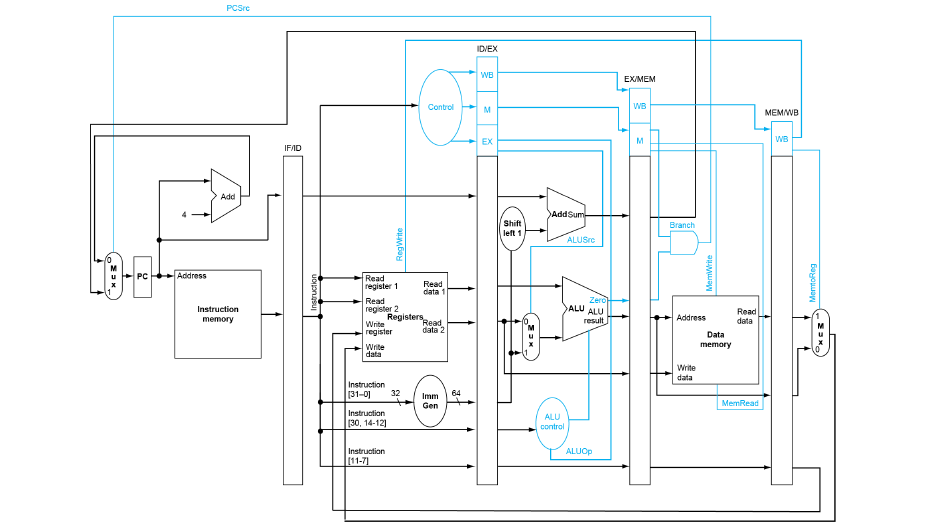
\includegraphics[width=18cm]{./images/structure}
	\caption{General structure}
	\label{fig2.1}
\end{figure}
As requested by the specifications, Instruction and Data memory are not included in the main architecture, however they are implemented it in the testbench.\\
Here we have tried to implement most of the single blocks in a Structural way. \\
Our approach was to describe, where possible, all blocks in a structural manner, so that some parts gain in performance (for instance the branch target adder is built using a CSEA structure instead of using the "+" operand inside a process).
Only Register File, ALU and all Filp-flops are implemented as Behavioral.\\
\\
On Figure \ref{fig2.2} it is showed how we have organized the VHDL files.
\begin{figure}[h!]
	\centering
	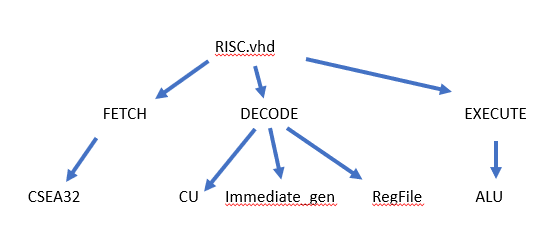
\includegraphics[width=15cm]{./images/VHDL_structure}
	\caption{General VHDL structure}
	\label{fig2.2}
\end{figure}
Now more details on the singular block implementation.
\section{Fetch}
\begin{figure}[h!]
	\centering
	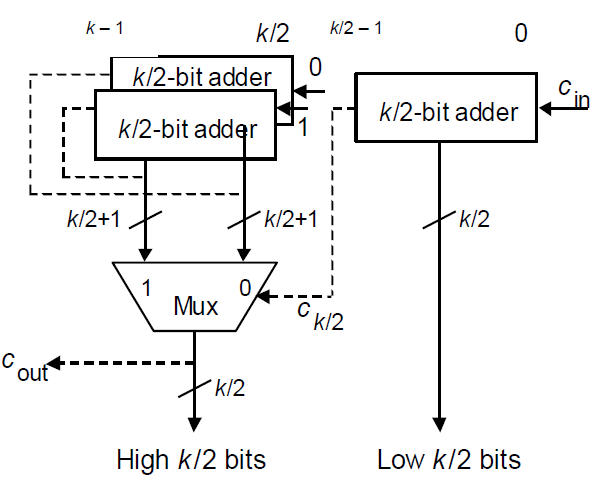
\includegraphics[width=10cm]{./images/CSEA}
	\caption{CSEA structure}
	\label{fig2.3}
\end{figure}
To update the PC we have implemented a Carry Select Adder. \\
Each singular block is composed of a 8 bit Ripple carry adder, in this way the carry propagation delay is reduced.
\section{Decode}
The register file is described in a behavioral manner and it is composed of 32 registers with 32 bit each.\\
When the instruction requires to write data, it will be available only at the next clock cycle in the register. On the other hand, a read operation from a register, is immediately available at the corresponding output.
Ports ReadRegister1 and ReadRegister2 are used to select (using the address at their inputs) a register for the read operation; same for the WriteRegister port that is used for write operations.\\
A write enable signal is used to tell when the RF has to write in the register location.
The register file has the following ports:
\begin{itemize}
	\item Register read1;
	\item Register read2;
	\item WriteRegister;
	\item WriteData;
	\item Read Data1;
	\item Read Data1;
	\item RegWrite;
	\item Reset;
	\item Clock;		
\end{itemize}

The Immediate\_generate block simply reads the instruction and generates a Immediate value (using bit extension).
\begin{figure}[h!]
	\centering
	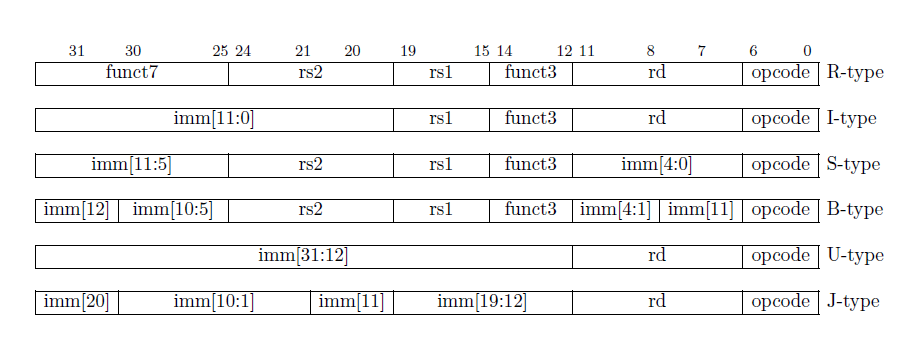
\includegraphics[width=10cm]{./images/immediate_gen}
	\caption{Instruction organization}
	\label{fig2.4}
\end{figure} 
So based on which instruction we are decoding, it organizes a 32 bits Immediate value.
Here we have placed the Control Unit, see next chapter for further details.
\section{Execute}
The adder that creates the new program counter is again implemented with a 32 bits CSEA.
Then we have the ALU that receives two inputs values and the Opcode specifies which instruction should be implemented.\\

In the second version of the processor (that implements the absolute value), we decided to to make the ALU perform the operation, given the proper instruction (that we called ABSV).
More details about the instruction ABSV are described in the Control Unit section of this report.\\

\section{Memory}
This module is described in the RISC top entity. It contains only the AND port that generates the selection signal for the multiplexer on the fetch phase.
\section{Write back}
This module is implemented in the RISC top entity. It contains a four inputs multiplexer and selects between:
\begin{itemize}
	\item Data memory read;
	\item Alu result;
	\item PC + 4 taken from fetch unit;
	\item PC where we need to jump;
\end{itemize}
The last two inputs are considered for the instruction AUIPC and JAL.
The JAL stores the address of the instruction following the jump (pc+4) into register rd.\\
So we take the updated PC in the fetch phase and we bring it in the Write Back phase.\\
AUIPC forms a 32-bit offset from the 20-bit U-immediate and adds this offset to the address of the AUIPC instruction.\\
Then places the result in register rd. 
We take the result in the Execute phase, where with the CSEA we create the branch PC.